\documentclass{article}
\usepackage{times}

\usepackage{amsmath}
\usepackage{amsfonts}
\usepackage{amssymb}
\usepackage{amsbsy}
\usepackage{caption}
\usepackage{chngcntr}
\usepackage{etoolbox}
\usepackage{graphicx}
\usepackage{hyperref}
\usepackage[margin=0.5in]{geometry}  % margins

\graphicspath{ {./figs/} }
\hypersetup{
    colorlinks=true,
    linkcolor=blue,
    filecolor=magenta,      
    urlcolor=cyan,
}

% reset eqn numbering in sub-sections
\numberwithin{equation}{section}

\begin{document}

\title{Technical Primer on A/B Testing}
\author{Ben Dundee\\Business Operations\\RetailMeNot, Inc.}
\date{\today}
\maketitle

\tableofcontents

\section{Introduction}

The goal of this document is to provide a technical introduction to the concepts behind AB testing for teams involved in planning/defining tests and analyzing their results. It's going to get mathy here... Section \ref{sec_stat_tests}, in particular, is math-heavy. If you're not inclined to follow along with the details, there's a bit at the end each section called ``What Does it Mean?'', where we attempt to relate all of the theoretical formalism back to the task at hand. That being said, a lot of technical details about the various statistical tests that we use in AB testing are included, mostly because I haven't found a good reference for this stuff myself. The goal is to equip the teams running these tests with the machinery to decide how tests should be designed.

\subsection{Why do we AB test?}
Tech companies test because they don't know how users will react to changes in their software. Writing and deploying code is cheap compared to the cost of acquiring new users, or the penalty incurred by alienating existing users. We need to understand: how will the business be impacted by specific changes?

Inherently, we're making a business decision about deploying (or not deploying) some change set. All of the math in this document is in service of that -- how are we to decide how things are likely to change, and how much confidence can we have in the results? The goal is to make informed decisions.

\subsection{How do we AB test?}
The procedure for testing an hypothesis has four steps. Once we've picked an experiment (take this as step 0!):
\begin{enumerate}
	\item Define null/alternative hypotheses. The null hypothesis is usually something like ``no effect exists''.
	\item Choose a statistic. This document describes four tests that are useful in AB testing, though there are a lot of other statistical tests that have been developed.
	\item Define a criteria for rejecting the null hypothesis. A test statistic implies a distribution, the distribution is used to set a decision criterion.
	\item Use test data to compute the value of the test statistic, and apply the criteria in (3) to make a decision about which hypothesis to reject.
\end{enumerate}
The goal of this document is to provide the technical details behind each of these steps, keeping in mind that the goal is to inform our final decision with data.

\subsection{Definitions and Assumptions \label{assumptions}}
We take the following definitions going forward:
\begin{itemize}
	\item $n_c \equiv $ number of sessions in the control slice;
	\item $n_t \equiv $ number of sessions in the test slice;
	\item $p_c \equiv$ the probability that a user performs a given action in the control slice; 
	\item $p_t \equiv$ the probability that a user performs a given action in the test slice.
\end{itemize}
For most tests, we can take the following assumptions:
\begin{itemize}
	\item \textbf{Large samples.} This means $n_c, n_t >> 1$, and in particular $n_c, n_t \sim \mathcal{O}\left(10^{5-6}\right)$.
	\item \textbf{Symmetry.} By construction, sample sizes are roughly the same: $n_c \approx n_t$. Where appropriate, we may define $\epsilon \equiv 1 - \frac{n_c}{n_t}$ (assuming $n_t$ is slightly larger than $n_c$), so that $\epsilon$ is positive definite and small.
	\item \textbf{Small effect sizes.} Effect sizes are typically small $\alpha \equiv 1 - \frac{p_c}{p_t}$ (assuming $p_c$ is smaller than $p_t$), so that $\alpha$ is positive definite and small. Typically, $\alpha \lesssim 5\% << 1$.
\end{itemize}
We'll refer to these assumptions throughout this document.

\subsubsection{When Do These Assumptions Not Apply?}

The assumptions we made above generally apply in AB testing, but we should be careful. In particular:
\begin{itemize}
	\item We may want to test a new experience on a very small set of users. This may occur during in-person tests of new UI patterns, for example. The Large Sample assumption should be relaxed if $n_c + n_t \lesssim 100$.
	\item Test slices may not be symmetric -- for example, if there's a bug in the software that affects the way users are sliced into test experiences. The Symmetry assumption should be relaxed if the difference in sizes between the two slices is $\gtrsim \frac{1}{100}$.
	\item Effect sizes may be large (this is typically a GOOD THING!). Note the assumption above that effects sizes change by $\lesssim 5\%$. Large movements in test metrics violate the above assumptions.\footnote{That being said, if you run a test and see a large movement in your core metrics, you likely don't need a statistical test to tell you the result is significant. }
\end{itemize}
These bounds are probably overly conservative -- generally, if you are testing in this range, you'll want to check the test stats against each other. In these cases, you'll want to favor Welch's test over the others, as it accommodates large differences in test/control variances and small sample sizes. And (as we'll show), when it \textit{doesn't} matter, Welch's test gives the same results as the other tests.

\section{Some Quick Background}

\subsection{Bernoulli Trials}
Most AB tests measure ratios -- the percentage of users who click or convert, for example. You can imagine this as follows: Each user who visits your site has a coin that has some probability $p$ of coming up heads. The user comes to the site, flips their coin, and if it comes up heads they click (or convert). This is called a ``Bernoulli Trial''.

Consider a sequence of $n$ coin flips, the results of which are encoded in random variables $X_i$. The coin lands on heads with probability $p$ and tails with probability $1-p$. For a single coin (taking $X_i = 1$ as heads and $X_i = 0$ as tails), the mean (expectation value) of $X_i$ is: 
\begin{equation} \label{bernoulli_mean}
	\mathbb{E}(X_i) = p
\end{equation}
and the variance of $X_i$ is 
\begin{equation} \label{bernoulli_var}	
	\mathrm{Var}(X_i) = \mathbb{E}(X_i^2) - \mathbb{E}^2(X_i) = p(1-p).
\end{equation}

We'll use these formulae implicitly in what follows -- in particular, we'll simply substitute the values in Equations (\ref{bernoulli_mean}) and (\ref{bernoulli_var}) for mean and variance in what follows. If you find it useful to think in terms of concrete terms, think of $X_i$ as an indicator that a user clicks (1 if they click, 0 if they do not), $p$ is the click-through ratio, and $n$ is the sample size.

\subsection{Population Statistics vs. Sample Statistics}

Consider a large population (say, all the gazelle in Zimbabwe). There exists exactly one answer to the question: ``What is the average mass of a gazelle in Zimbabwe?''. Likewise, there is exactly one answer to the question: ``What is the standard deviation of the masses of all the gazelle in Zimbabwe?''.  

The distinction here is between quantities measured across the entire population (``population mean'' and ``population variance'') and quantities measured across a \textit{sample} of the population (``sample mean'' and ``sample variance''). The notation is as follows:
\begin{itemize}
	\item The mass of one gazelle is $m_g$, the average mass of \textit{all} gazelle is $\mathbb{E}(m_g) = \mu$. There is one, and only one right answer. We've measured the mass of every gazelle in this example, and $\mu$ is a ``population statistic'' because we average across the entire population.
	\item Likewise, the variance of all gazelle masses is $\mathrm{Var}(m_g) = \sigma^2$. $\sigma^2$ is the ``population variance''.
	\item Suppose we were to take a sample of gazelle, and measure their masses. To make it clear that the number we have is the result of a single measurement, we write the average as $\mathbb{E}(m_g) = \hat{\mu}$, where the hat $\hat{ }$ denotes a measured quantity. We call $\hat{\mu}$ the ``sample mean'' because it's an average over a sample (subset) of the population.
	\item Likewise, if we were to measure the variance of the masses of the gazelle population, we write $\mathrm{Var}(m_g) = \hat{\sigma}^2$. This is called the ``sample variance''.
\end{itemize}

\subsection{Measurement Error (Standard Error of the Mean)}

It's worth noting that $\hat{\mu}$ and $\hat{\sigma}^2$ are \textit{measurements}, and so they're inherently random quantities. We can perform the same experiment multiple times and get different values each time.

Suppose we wanted to be very accurate in our gazelle assessment, so we set out to measure several samples of the population. In other words, we take a sample of gazelle from some part of the country and compute the sample's mean, we find $\hat{\mu}_1$. We repeat this process $N$ times, so that we have $\hat{\mathcal{M}} = \left\lbrace\hat{\mu}_1,\hat{\mu}_2,\ldots,\hat{\mu}_N\right\rbrace$.

How are we to report our results? To get an idea of the mass, we can simply take the average:
\begin{equation}
	\mathbb{E}(\hat{\mathcal{M}}) = \frac{1}{N}\left(\hat{\mu}_1 + \hat{\mu}_2 + \cdots + \hat{\mu}_N\right).
\end{equation}
If our experiments are fair (``unbiased''), then we expect:
\begin{equation}
	\mathbb{E}(\hat{\mathcal{M}}) = \mu \Rightarrow \mathbb{E}(\hat{\mathcal{M}}) - \mu = 0,
\end{equation}
This last condition amounts to saying that ``$\hat{\mathcal{M}}$ is a good estimator of $\mu$'', or ``$\hat{\mathcal{M}}$ is an unbiased estimator of $\mu$''.

What about the variance of $\hat{\mathcal{M}}$? Each $\hat{\mu}_i$ is a random variable, drawn from a population whose variance is $\sigma^2$. We define the ``standard error of the mean'' ($s$) as the standard deviation of $\hat{\mathcal{M}}$. The variance of $\hat{\mathcal{M}}$ is:
\begin{equation}
	\mathrm{Var}\left(\hat{\mathcal{M}}\right) = \mathrm{Var}\left(\frac{1}{N}\sum_i^N \hat{\mu}_i\right) = \frac{1}{N^2}\sum_i^N \mathrm{Var}(\hat{\mu}) = \frac{N\times\hat{\sigma}^2}{N^2} = \frac{\hat{\sigma}^2}{N}.
\end{equation}
Thus, the standard error is given by:
\begin{equation} \label{std_error}
	\hat{s} \equiv \frac{\hat{\sigma}}{\sqrt{N}}.
\end{equation}

Note that Equation (\ref{std_error}) is defined in terms of the sample statistic $\hat{\sigma}$, so it's an \textit{estimate}. Ideally we'd use the population standard deviation, but in this case, an estimate is the best that we can do. As we expect, the measurement error goes to 0 as we take larger and larger sample sizes.

\section{Hypothesis Building}

Defining the hypothesis at the start of an experiment is something lots of people brush off. In particular, hypotheses are often stated as ``The new call-to-action (CTA) will drive conversion''. Why will the new CTA drive conversion? What makes us think that this drives conversion higher vs. lower? Why should we run this test over the other 50 tests we could be running? As analysts/scientists, it is up to us to hold business owners accountable for defining what is being tested, what the result is likely to be, and why we're bothering running the test in the first place. 

\subsection{Informal Definition of the Hypothesis}

Business owners need a way to define hypotheses in language they understand, in a way that allows the analyst to map that back to a well-defined null/alternative hypotheses. To that end, we've found the following template to be successful\footnote{For example: https://blog.optimizely.com/2015/01/29/why-an-experiment-without-a-hypothesis-is-dead-on-arrival/}:
\begin{itemize}
	\item If [description of change], then [expected outcome] because [assumption to be tested].
\end{itemize}
It's common for stakeholders to be very loose when it comes to defining hypotheses for experiments. This format is easy to understand, and puts the onus on business partners to come up with what effect they believe their changes will drive. Crucially, it ensures that business owners can justify their assertion, and serves as a starting place for analysts to draw connections across several tests.

\subsection{Formal Definition of the Hypothesis \label{sec_hypothesis}}

Once we have the informal statement of the hypothesis, we can build a formal set of hypotheses to test. We're focusing on AB tests here, so there are two hypotheses:
\begin{itemize}
	\item The Null Hypothesis ($\mathcal{H}_0$) generally assumes that no effect is present.
	\item The Alternative Hypothesis ($\mathcal{H}_1$) assumes that the Null Hypothesis is incorrect.
\end{itemize}
A few quick comments:
\begin{itemize}
	\item The two hypotheses are mutually exclusive. Both cannot be simultaneously true.
	\item Ideally, you will design experiments such that your hypotheses are testing exactly one change. If you do not do this and your experiment rejects $\mathcal{H}_0$, you will lose the ability to understand which change caused the effect. Think of it this way, if you try to change two things and run one test, you'll still need to run another test anyway to disambiguate the results. If you can't get to the core driver of the change in your test metrics, you can't get at the user behavior. And the user behavior is what we're supposed to be measuring!
	\item The Alternative Hypothesis can either be ``one tailed'' or ``two tailed''. This is important when it comes to setting a threshold for accepting or rejecting the Null Hypothesis, it will be discussed in more detail in Section \ref{sec_threshold}.
\end{itemize}

\subsubsection{Choosing a Test Metric}
The hypothesis that you get from your stakeholder should allow you to pick a test metric. In what follows, we assume the metric is a number that you can consistently and repeatedly measure. There should be no doubt about why the number is important, or about how to calculate the number in the first place. This test metric forms the basis of your hypothesis.

For example, if we're testing a new CTA, we might expect to increase click-through ratio (CTR), $c$. We split our site traffic into two cohorts, and apply the treatment (in this case, ``new and improved'' CTA) to half of it. This is the test slice. The Null and Alternative Hypotheses might be:
\begin{eqnarray}
	\mathcal{H}_0 &:& c_c = c_t \\
	\mathcal{H}_1 &:& c_c < c_t.
\end{eqnarray}
In English: 
\begin{itemize}
	\item The Null Hypothesis states that the treatment has no effect, and that the CTR in both cases will be the same.
	\item The Alternative Hypothesis states that the treatment, applied to the test slice, drove a higher CTR.
\end{itemize}

This test is ``one tailed'', in the sense that you're looking for an improvement in CTR. You may also define a ``two tailed'' test:
\begin{eqnarray}
	\mathcal{H}_0 &:& c_c = c_t \\
	\mathcal{H}_1 &:& c_c \neq c_t.
\end{eqnarray}
Here, the Alternative Hypothesis states that the CTR in the test slice is \textit{different} from the control slice. There is a subtle difference between these two sets of hypotheses that we'll discuss in Section \ref{sec_threshold}.

\section{Statistical Tests \label{sec_stat_tests}}

There is a lot of information about hypothesis testing available online. A lot of it is hard to understand, or misleading. I hope that this section clarifies things somewhat. In particular, I wanted to derive the $Z$ test from first principles, to understand what assumptions are being made, where those assumptions make sense, and where they bite you.

\subsection{Properties of Statistical Tests}

For our purposes, a statistical test is a way to assess a measurement in a way that allows one to compare that result against likely outcomes. This means we have to have a way to understand ``likely'', which implies some distribution of possibilities. The test statistic $t$ is defined in terms of measured quantities, so the test statistic \textit{implies} a distribution of outcomes. We will consider three types of tests in what follows:
\begin{enumerate}
	\item The $Z$ test. The test statistic, $t_Z$ has a normal distribution with mean 0 and variance 1.
	\item The $t$ test. The test statistic, $t_t$ follows a Student's $t$ distribution with $n_c + n_t - 2$ degrees of freedom.
	\item Welch's $t$ test. The test statistic $t_W$ follows a Student $t$ distribution with $d_W$ degrees of freedom. We'll define $d_W$ below, but $d_W \neq n_c + n_t - 2$ generally.
\end{enumerate}
In this section, we'll outline the main differences between the three, and when those differences matter.

The test statistics that we discuss here have the same form:
\begin{equation} \label{general_t_stat}
	t = \frac{\hat{p}_c - \hat{p}_t}{\hat{s}},
\end{equation}
where $\hat{s}$ is the standard error. The difference between all of the tests that we discuss comes down to how we estimate the standard error, $\hat{s}$. Biases in the estimates produce shifts in $t$, which affect the decisions that are made about significance. We'll attempt to quantify these biases below, to give a sense of how much each of the $t$ stats we use are affected.

\subsubsection{Aside: What is Bias, and How Does Bias Affect $t$?}

In what follows, we compute the bias in the standard error to understand how our assumptions affect the value of $t$ we use for our tests. The bias $b$ of the standard error $s^2$ is defined as:
\begin{equation}
	b \equiv \mathbb{E}(\hat{s}^2) - s^2.
\end{equation}
Note that we're taking the expectation value over the \textit{estimated} $\hat{s}^2$, which is written in terms of the sample variance, and comparing it to $s^2$, which is written in terms of the population variance. We have to assume that we know both quantities in order to compute $b$.

If we use a biased $\hat{s}^2$, our $t$ will be biased. We can compute how much $t$ will change, based on the bias implicit in our strategy to estimate $\hat{s}$:
\begin{equation}
	t_{\mathrm{bias}} = \frac{\hat{p}_c - \hat{p}_t}{\hat{s}_{\mathrm{bias}}^2}.
\end{equation}
To correct for the bias in $\hat{s}^2_{\mathrm{bias}}$:
\begin{equation}
	t_{\mathrm{bias}} = \frac{\hat{p}_c - \hat{p}_t}{\hat{s}^2 + b}.
\end{equation}
If we assume bias is small (a good assumption, see below), then we can write the \textit{unbiased} value of $t$ as:
\begin{eqnarray} \nonumber \label{biased_t}
	t_{\mathrm{bias}} &=& \frac{\hat{p}_c - \hat{p}_t}{\hat{s}^2} \times \left(1 - \frac{b}{\hat{s}^2}\right) + \mathcal{O}(b^2) \\
	\Rightarrow t_{\mathrm{bias}} &=& t \times \left(1 - \frac{b}{\hat{s}^2}\right) = t \times \left(1 - \frac{b\sqrt{N}}{\hat{\sigma}^2}\right).
\end{eqnarray}

Equation (\ref{biased_t}) gives us a way to understand how the bias in our estimator $\hat{s}^2$ affects the value of $t$ that we calculate. When bias is large, the corrections to our $t$ stat are large. Likewise, if we're working in a regime where bias is small, the corrections to the $t$ stat are small. This is an important point, because the value of $t$ dictates the decision we make on a test -- if $t$ is greater than some threshold (see Section \ref{sec_threshold}), we agree to reject the Null Hypothesis. If the shift in $t$ caused by the bias in our estimator $\hat{s}^2$ is small, the decision we make about rejecting or accepting the Null Hypothesis is unaffected.

\subsection{$Z$ Test \label{sec_z_test}}

In order to determine the correct statistic, start with the null hypothesis. For an AB test, we hypothesize that there is no effect, and that the means of the control and test slice are the same:
\begin{equation} \label{null_hypothesis}
	\mathcal{H}_0: p_c = p_t.
\end{equation}
The null hypothesis says that the treatment in the test slice has no effect. If the null hypothesis is correct, then $p_c = p_t = p$, where $p$ is the population mean. 

Suppose we go out and measure $p_c$ and $p_t$. Our measurements, $\hat{p}_c$ and $\hat{p}_t$, should be good \textit{estimates} of $p_c$ and $p_t$. This means
\begin{eqnarray}  \nonumber \label{unbiased_estimators}
	\mathbb{E}(\hat{p}_c) - p_c &=& 0 \\
	\mathbb{E}(\hat{p}_t) - p_t &=& 0
\end{eqnarray}
The quantities $\hat{p}_c$ and $\hat{p}_t$ are called ``unbiased estimators'' of $p_c$ and $p_t$. ``Unbiased'' means Equations (\ref{unbiased_estimators}) hold. It's the same as saying: ``If we were to perform the experiment many times, average all the results together, \textit{and} the null hypothesis were true, we'd find $\mathbb{E}\left(\hat{p}_c\right) = p_c$ and $\mathbb{E}\left(\hat{p}_t\right) = p_t$.'' Subtracting Equations (\ref{unbiased_estimators}), we find:
\begin{eqnarray} \label{z_num} \nonumber
	\mathbb{E}\left(\hat{p}_c - \hat{p}_t\right) - \left(p_c - p_t\right) &=& 0 \\
	\Rightarrow \mathbb{E}\left(\hat{p}_c - \hat{p}_t\right) &=& 0.
\end{eqnarray}
The quantity $\hat{p}_c - \hat{p}_t$ has a normal distribution with mean zero, if the null hypothesis is true. 

The standard error can be written in terms of the variance:
\begin{eqnarray} \nonumber \label{z_denom_pre}
	\hat{s}^2 &=& \frac{\hat{p}_c(1-\hat{p}_c)}{n_c} + \frac{\hat{p}_t(1-\hat{p}_t)}{n_t}, \\ 
	\Rightarrow \hat{s}^2 &=& \hat{p}(1-\hat{p}) \left(\frac{1}{n_c} + \frac{1}{n_t}\right).
\end{eqnarray}
Equation (\ref{z_denom_pre}) quantifies the uncertainty in the measurement in terms of (an estimate of) the population mean $\hat{p}$. In terms of measured quantities:
\begin{equation} \label{p_hat}
	\hat{p} = \frac{n_t \hat{p}_t + n_c \hat{p_c}}{n_t + n_c}.
\end{equation}
If $\hat{p}_c$ is an unbiased estimator of $p_c$, and $\hat{p}_t$ is an unbiased estimator of $p_t$, then you can easily show that $\hat{p}$ in Equation (\ref{p_hat}) is an unbiased estimator of $p$, \textit{assuming the variance in the control and test group are the same}. (We'll come back to this point below.) So the \textit{estimate} of our error in terms of the \textit{sample} variance is
\begin{equation} \label{z_denom}
	\hat{s}^2 = \hat{p}(1-\hat{p}) \left(\frac{1}{n_c} + \frac{1}{n_t}\right).
\end{equation}

Using Equations (\ref{z_num}), (\ref{p_hat}), and (\ref{z_denom}) in (\ref{general_t_stat}), we find:
\begin{equation} \label{z_test_stat}
	t_z \equiv \frac{\hat{p}_c - \hat{p}_t}{\sqrt{\hat{p}\left(1-\hat{p}\right)\times\left(\frac{1}{n_c} + \frac{1}{n_t}\right)}}.
\end{equation}
Note that the right hand side of Equation (\ref{z_test_stat}) is written entirely in terms of \textit{measured} quantities.

\subsubsection{Confusion}

I've always been confused by Equation (\ref{z_denom}). Why do we need $p$ in the first place? The only way we can know anything about it is by writing it in terms of some other things that we have to measure anyway. I've found no good explanations for the substitution that we made in Equation (\ref{z_denom}). 

Suppose we \textit{didn't} make the substitution in Equation (\ref{z_denom}), and stopped one step sooner. Then we'd just use:
\begin{equation} \label{alternative_z_denom}
	\hat{s}^2 = \frac{\hat{p}_c(1-\hat{p}_c)}{n_c} + \frac{\hat{p}_t(1-\hat{p}_t)}{n_t}.
\end{equation}
The resulting $t$ stat is:
\begin{equation} \label{alternative_z_stat}
	t_{z'} = \frac{\hat{p}_c - \hat{p}_t}{\sqrt{\frac{\hat{p}_c(1-\hat{p}_c)}{n_c} + \frac{\hat{p}_t(1-\hat{p}_t)}{n_t}}}.
\end{equation}
Theoretically, whether we choose to use Equation (\ref{z_test_stat}) or (\ref{alternative_z_stat}) is a choice made by the experiment designer. Both equations are valid, and reduce to the same result given that the null hypothesis is true.

The interesting thing is that Equation (\ref{alternative_z_stat}) results in a very similar $t$ statistic that you get from Welch's test, see Equation (\ref{welchs_t_stat}). In particular, we never had to assume anything about the variances in test/control slice to get Equation (\ref{alternative_z_stat}). That test implies a different underlying distribution, which affects step (3) in our hypothesis testing procedure, where we set a criteria for accepting or rejecting the null hypothesis.

\subsubsection{Computing the Bias}
In Equations (\ref{z_denom}), we've assumed that the variance of the test and control slices were the same. Here, we'll show to what extent the estimates that we made based on that assumption are good estimates by computing the bias. 

First, we argued above that $\hat{p}_c$ and $\hat{p}_t$ were unbiased estimators of $p_c$ and $p_t$, and that $\mathbb{E}(\hat{p}_c - \hat{p}_t) = 0$. If we knew $p_c$ and $p_t$, then we'd \textit{know} the measurement error:
\begin{equation}
	s^2 = \mathrm{Var}\left(\hat{p}_c - \hat{p}_t\right) = \frac{p_c(1-p_c)}{n_c} + \frac{p_t(1-p_t)}{n_t}
\end{equation}
Assuming a common variance across $p_c$ and $p_t$:
\begin{equation}
	\hat{s}_0^2 = \hat{p}(1-\hat{p})\left(\frac{1}{n_c} + \frac{1}{n_t}\right).
\end{equation}
The bias in the estimate of the standard error is
\begin{equation} \label{bias}
	b = \mathbb{E}\left(\hat{s}^2_0\right) - s^2.
\end{equation}
We define $\Delta \equiv p_t - p_c$ and $N \equiv n_c + n_t$, then:
\begin{eqnarray}
	p - p_c &\equiv& \frac{n_t}{N} \Delta, \\
	p - p_t &\equiv& -\frac{n_c}{N}\Delta.
\end{eqnarray}
Note that $\Delta \sim \mathcal{O}(\alpha)$. Writing Equation (\ref{bias}) in terms of $\Delta$, I find:
\begin{equation} \label{z_score_bias}
	b = \frac{\Delta}{N}\left[\frac{n_t}{n_c} \left(1-p-p_c\right) + \frac{n_c}{n_t} \left(1-p-p_t\right)\right].
\end{equation} 
As expected, if $p = p_c = p_t$, $\Delta = 0$ and the bias is zero. But consider Equation (\ref{z_score_bias}) in light of the our AB testing assumptions in Section \ref{assumptions} -- we test in a region where $n_c \approx n_t$, and $n_c, n_t, N >> 1$. This implies:
\begin{equation} \label{z_score_bias_scaling}
	b \sim \frac{1}{N}\left[\mathcal{O}(\epsilon) + \mathcal{O}(\alpha)\right]
\end{equation}
Since bias scales like $\frac{1}{N}$, corrections to the $t$ stat scale like $\frac{1}{\sqrt{N}}$, see Equation (\ref{biased_t}). The point is that the bias introduced by treating the underlying sample variances as equal in this regime is negligible. 

\subsubsection{What Does it Mean?}

The main goal of all of this theoretical development is to give us some intuition about when the $Z$ test is valid to use, and when you should use a different test. In this section, we've shown that the $Z$ test is robust enough to be used in most AB testing situations. If we want to relax our assumptions, we have shown that corrections to $t_Z$ are small ($\sim \mathcal{O}\left(\frac{\alpha}{\sqrt{N}}\right) + \mathcal{O}\left(\frac{\epsilon}{\sqrt{N}}\right)$). In particular, we've shown that the $Z$ test is valid when our core assumptions apply:
\begin{itemize}
	\item Large samples;
	\item Symmetry; 
	\item Small effects.
\end{itemize}
All of the quantities that we've used to derive Equations (\ref{alternative_z_stat}) (and (\ref{z_test_stat})) are valid in this regime. In the following sections, we will establish that both Student's $t$ test and Welch's $t$ test reduce to the $Z$ test under our assumptions.

\subsection{Student's $t$ Test}

It turns out that Equations (\ref{z_denom}) and (\ref{alternative_z_denom}) actually produce \textit{biased} estimates of the true variance. Intuitively, you can see why by considering an experiment where $n_c, n_t \sim \mathcal{O}(1)$. In that case, you're much more likely to sample the center of the distribution, and much less likely to sample the tails. This means that, while you'll do a good job of estimating the population mean, you'll end up \textit{underestimating} the population variance. In order to get a good test statistic, you have to correct for the bias introduced by a small sample size. You do this by finding a better way to estimate variance, and using a distribution that is less sharply peaked -- it has ``fatter tails''. This is the Student's $t$ distribution.

It can be shown that a good estimate of the population variance can be obtained by taking a weighted average of the sample variances, which is called the ``pooled variance'':
\begin{equation} \label{pooled_variance}
	\hat{\sigma}_p^2 = \frac{\left(n_c - 1\right) \hat{\sigma}_c^2 + \left(n_t - 1\right) \hat{\sigma}_t^2}{n_c + n_t - 2}.
\end{equation}
It's clear, from Equation (\ref{pooled_variance}), that this only really matters when $n_c, n_t \sim \mathcal{O}(1)$. If $n_c, n_t >> 1$, then $n_c - 1 \approx n_c$ and $n_t - 1 \approx n_t$, and Equation (\ref{pooled_variance}) reduces to Equation (\ref{z_denom}) under the null hypothesis.

Plugging this in to our general $t$ stat in Equation (\ref{general_t_stat}), we get Student's $t$ test statistic:
\begin{equation} \label{student_t_stat}
	t_t = \frac{\hat{p}_c - \hat{p}_t}{\sqrt{\hat{\sigma}_p^2\left(\frac{1}{n_c} + \frac{1}{n_t}\right)}}.
\end{equation}
The underlying distribution implied by this test is Student's $t$ distribution, with $n_c + n_t - 2$ degrees of freedom.\footnote{An easy way to understand the sudden appearance of $n_c-1$ and $n_t-1$ is to consider an experiment with $n_c = 1$ and $n_t = 1$. In that case, you can get an estimate of the population mean (in this case, 1 or 0), but you can't get an estimate of the variance -- the variance \textit{requires} that you have multiple measurements, if you have a single measurement the variance is undefined. (It's a bit confusing in our case because the variance is defined in terms of the mean, $p$.) The factor $n-1$ is called ``Bessel's correction'', and can be understood in several other ways. A good visual example can be found at https://www.khanacademy.org/computer-programming/fishy-statistics-unbiased-estimate-of-population-variance/1183564841.}

\subsubsection{Pooled Variance: Asymptotic Behavior}
Under the assumptions laid out in the first section, we'd like to understand what happens to $t_t$ in the limit where sample sizes are large and (roughly) equal, and effect sizes are small. This amounts to expanding Equations (\ref{student_t_stat}) and (\ref{pooled_variance}) in $\alpha$ and $\epsilon$.

First, we write:
\begin{equation}
	\hat{\sigma}_p^2 = \left(\frac{n_c}{n_c + n_t}\right) \hat{\sigma}_c^2 \left[1 + \frac{n_t^2}{n_c^2}\frac{\hat{\sigma}_t^2}{\hat{\sigma}_c^2}\right],
\end{equation}
where we've used $n_{c,t} - 1 \approx n_{c,t}$. Substituting $\hat{p}_c = \left(1-\alpha\right) \hat{p}_t$ and $n_c = \left(1-\epsilon\right) n_t$, we find
\begin{eqnarray} \nonumber \label{pooled_var_large_n}
	\hat{\sigma}_p^2 &=& \left(\frac{n_c \hat{\sigma}_c^2}{2n_c}\right) \times \left[1 + \left(1 + \mathcal{O}(\alpha)\right)\times\left(1 + \mathcal{O}(\epsilon)\right)\right] \\
	\hat{\sigma}_p^2 &=& \hat{\sigma}_c^2 + \mathcal{O}(\alpha) + \mathcal{O}(\epsilon).
\end{eqnarray}
Equivalently, we could have written 
\begin{equation} \label{pooled_var_large_n_alt}
	\hat{\sigma}_p^2 = \hat{\sigma}_t^2 + \mathcal{O}(\alpha) + \mathcal{O}(\epsilon).
\end{equation}
Thus, under the assumptions in Section \ref{assumptions},
\begin{equation} \label{pooled_var_large_n_final}
	\hat{\sigma}_p\sqrt{\frac{1}{n_c} + \frac{1}{n_t}} \approx \sqrt{\frac{\hat{\sigma}_c^2}{n_c} + \frac{\hat{\sigma}^2_t}{n_t}}.
\end{equation}

So what do Equations (\ref{pooled_var_large_n}) and (\ref{pooled_var_large_n_alt}) \textit{mean}? Basically, if your AB test follows the assumptions listed at the beginning of this doc, the pooled variance is equal to the variance in the control slice (which is roughly equal to the variance in the test slice, which is roughly equal to the population variance, if we believe the null hypothesis to be true), up to small corrections. 

This is expected -- at the beginning of this section, we described why the estimates in Equations (\ref{z_denom}) and (\ref{alternative_z_denom}) were biased. The bias only appears for small sample sizes (i.e., when you don't have enough measurements to ensure that you're sampling the tails of the distribution). Thus, it should be no surprise that this bias disappears when sample sizes are large, as in Equation (\ref{pooled_var_large_n}).

Finally, the $t$ stat in Equation (\ref{student_t_stat}) and the $Z$ stat in Equation (\ref{alternative_z_stat}) have the same form, up to small corrections. But while they have the same form, they still imply different distributions. In the next section, we'll show what the Student's $t$ distribution looks like, under the assumptions in Section \ref{assumptions}.

\subsubsection{Student's $t$ Distribution: Asymptotic Behavior \label{sec_student_t_asymp}}
We now ask, in our testing regime, what does the $t$ distribution look like, given that we have very large sample sizes? Recall: Step (3) in the process requires that you know the distribution (which is fully specified by the density) to set a confidence level. For $n$ degrees of freedom, we have
\begin{equation} \label{student_t}
	f_n(x) = \frac{\Gamma\left(\frac{n+1}{2}\right)}{\sqrt{\pi n} \Gamma\left(\frac{n}{2}\right)}\left(1+\frac{x^2}{n}\right)^{-\frac{n+1}{2}},
\end{equation}
where $\Gamma$ is Euler's gamma function. ``Degrees of freedom'' means ``number of trials'', so our assumptions (Large Samples) imply $n\rightarrow\infty$. To examine the limit, we note the following property of limits: 
\begin{equation}
	\lim_{x\rightarrow a} \left(g(x) h(x)\right) = \lim_{x\rightarrow a}  g(x) \times  \lim_{x\rightarrow a} h(x)\,
\end{equation}
under the assumptions that limits of $g$ and $h$ exist. Taking the limit of Equation (\ref{student_t}), we write:
\begin{eqnarray} \label{student_t_large_n} \nonumber
	\lim_{n\rightarrow \infty}f_n(x) &=& \lim_{n\rightarrow \infty} \frac{\Gamma\left(\frac{n+1}{2}\right)}{\sqrt{\pi n} \Gamma\left(\frac{n}{2}\right)} \times \lim_{n\rightarrow \infty} \left(1+\frac{x^2}{n}\right)^{-\frac{n+1}{2}}, \\
   	\Rightarrow \lim_{n\rightarrow \infty}f_n(x) &=& \mathcal{L}_1 \times \mathcal{L}_2.
\end{eqnarray}
Attacking these separately, the second limit looks familiar:
\begin{eqnarray} \label{second_part}
	\nonumber \mathcal{L}_2 = \lim_{n\rightarrow \infty} \left(1+\frac{x^2}{n}\right)^{-\frac{n+1}{2}}  &=& \lim_{n\rightarrow \infty} \left(1+\frac{x^2}{n}\right)^{-\frac{n}{2}} \times \lim_{n\rightarrow \infty} \left(1+\frac{x^2}{n}\right)^{-\frac{1}{2}}, \\
	\Rightarrow \mathcal{L}_2 &=& e^{-\frac{x^2}{2}}.
\end{eqnarray}
$\mathcal{L}_1$ requires the following identity of $\Gamma$:
\begin{equation} \label{useful_identity}
	\lim_{n\rightarrow \infty} \frac{\Gamma(m+\beta)}{\Gamma(m) m^\beta} = 1.
\end{equation}
Then we have:
\begin{equation} \label{first_part} 
	\mathcal{L}_1= \lim_{n\rightarrow \infty} \frac{\Gamma\left(\frac{n+1}{2}\right)}{\sqrt{\pi n} \Gamma\left(\frac{n}{2}\right)} =  \frac{1}{\sqrt{2\pi}}\lim_{n\rightarrow \infty} \frac{\Gamma\left(\frac{n}{2}+\frac{1}{2}\right)}{\left(\frac{n}{2}\right)^{\frac{1}{2}} \Gamma\left(\frac{n}{2}\right)} = \frac{1}{\sqrt{2\pi}}.
\end{equation}
Putting Equations (\ref{first_part}) and (\ref{second_part}) together, we see Equation (\ref{student_t_large_n}) becomes:
\begin{equation} \label{student_t_dist_becomes_normal}
	\lim_{n\rightarrow \infty}f_n(x) = \frac{1}{\sqrt{2\pi}} e^{-\frac{x^2}{2}},
\end{equation}
which is exactly the probability density of the normal distribution with mean zero and unit variance. Thus, we conclude, for large sample sizes (as is the case with our A/B tests), Student's $t$ distribution is approximately normal.

\subsubsection{What Does This Mean?}
Equation (\ref{student_t_stat}) bears a strong resemblance to Equation (\ref{z_test_stat}), given the result in Equation (\ref{pooled_var_large_n}). Indeed, the results in Section \ref{sec_z_test} might have given us this suspicion. But this is only half of the story. We also needed to establish that Student's $t$ distribution tended towards a normal distribution, which is the result in Equation (\ref{student_t_dist_becomes_normal}).  So:
\begin{itemize}
	\item The statistic $t_t$ in Equation (\ref{student_t_stat}) becomes indistinguishable from the statistic $t_Z$ in Equation (\ref{z_test_stat}) under the assumptions laid out in Section \ref{assumptions}. This is established in Equation (\ref{pooled_var_large_n_final}).
	\item The distribution implied by $t_t$ is the same as the test criteria is normal under the assumptions in Section \ref{assumptions}, the same as implied by the $Z$ test. This is established by Equation (\ref{student_t_dist_becomes_normal}).
\end{itemize}
Thus, under our assumptions, there is no practical difference between the $t$ test and the $Z$ test. In other words: Using a $Z$ test in the regime implied by our assumptions would lead to all the same testing decisions as using the $t$ test.

\subsection{Welch's $t$ Test}
To this point, we've made the assumption that the variances in the test and control slices are the same. We've argued that the bias introduced by this approximation scales as $\frac{\Delta}{N}$, where $\Delta \equiv p_c - p_t$ and $N$ is the sample size, see Equation (\ref{z_score_bias}). The pooled variance controls for this bias somewhat -- we won't show it here, but that bias introduced by using the pooled variance (which assumes the same variance across test and control slices) scales like $\frac{\hat{\sigma}_c^2 - \hat{\sigma}^2_t}{N}\times\mathcal{O}(\epsilon) \sim \frac{1}{N} \times \mathcal{O}(\alpha) \times \mathcal{O}(\epsilon)$, which is an order of magnitude smaller than what we found in Equation (\ref{z_score_bias_scaling}). 

For an A/B test with two slices, we define the following test statistic:
\begin{equation} \label{welchs_t_stat}
	t_W = \frac{\hat{p}_c - \hat{p}_t}{\sqrt{\frac{\hat{\sigma}_c^2}{n_c} + \frac{\hat{\sigma}_t^2}{n_t}}}
\end{equation}
The test statistic is then compared to Student's $t$ distribution with the following number of degrees of freedom:
\begin{equation} \label{welchs_dof}
	d_W \approx \frac{\left(\frac{\hat{\sigma}_c^2}{n_c} + \frac{\hat{\sigma}_t^2}{n_t}\right)^2}{\frac{\hat{\sigma}_c^4}{n_c^2 \left(n_c-1\right)} + \frac{\hat{\sigma}_t^4}{n_t^2 \left(n_t- 1\right)}}
\end{equation}
Note that $d_W$ is not strictly an integer. In order to do computations, you normally round this number.

\subsubsection{Welch's $t$: Asymptotic Behavior}
Compare Equation (\ref{welchs_t_stat}) to Equation (\ref{alternative_z_stat}). Given that $\hat{\sigma}_{c, t}^2 = \hat{p}_{c, t}(1-\hat{p}_{c, t})$, the two expressions are exactly the same! The only difference is in the distribution -- Welch's $t$ test directs us to set our threshold for rejecting the null hypothesis using Student's $t$ distribution, with $d_W$ degrees of freedom. But consider our assumptions in Section \ref{assumptions}. If we take $n_c \approx n_t \sim N >> 1$, then we can extract the scaling behavior of $d_W$:
\begin{eqnarray} \nonumber \label{nu_w_large_n}
	d_W &\sim& \frac{\frac{1}{N^2} \left(\hat{\sigma}_c^2 + \hat{\sigma}_t^2\right)^2}{\frac{1}{N^3}\left(\hat{\sigma}_c^4 + \hat{\sigma}_t^4\right)}, \\
	\Rightarrow d_W &\sim& N \times f\left(\hat{\sigma}^2_c, \hat{\sigma}^2_t\right).
\end{eqnarray}
Thus, $d_W$ scales as $N$. In the large $N$ limit, we've already shown that Student's $t$ distribution is normal, see Section \ref{sec_student_t_asymp}. Again we find that Welch's $t$ test reduces to the $Z$ test under the assumptions in Section \ref{assumptions}! This is not unexpected, as we showed that corrections to the $Z$ test had to be small, given the regimes where we were testing.

\subsection{Conclusion: Which Statistical Test Should I Use?}

It's likely that this is the only question you care about :) At the end of the day, we've shown the following in this section:
\begin{itemize}
	\item Student's $t$ test is appropriate to use when the sample size is small, and the variances in the test and control group are similar.
	\item Welch's $t$ test is appropriate to use when the sample size is small, and the variances in the test and control slices are different.
	\item Both tests reduce to the $Z$ test under the assumptions in Section \ref{assumptions}. Subject to those assumptions, it is true that $t_Z \approx t_t \approx t_W$, and that the distributions implied by all three test statistics are normal.
\end{itemize}
Based on (3), we conclude that the differences between the three tests are marginal in the regions we're likely to be testing in. Any of the three tests can be justified, the choice is left to the experiment designer.

\section{Setting the Threshold \label{sec_threshold}}

Once we've built our hypotheses and defined a test statistic, the next step is to determine a threshold for accepting or rejecting the Null Hypothesis. In designing our experiment, there are four possible outcomes. The Null Hypothesis can be either right or wrong, and our experiment can either accept or reject it. In two outcomes, we pick correctly, and our test will rightly accept or reject the Null Hypothesis. It's also possible that we make an error  -- if the Null Hypothesis is true and we reject it, we commit a Type I error, and if the Null Hypothesis is false and we accept in, we commit a Type II error. Let's define two parameters:
\begin{itemize}
	\item The probability that we incorrectly reject the null hypothesis (commit a Type I error) is $a$; and
	\item The probability that we incorrectly accept the null hypothesis (commit a Type II error) is $b$.
\end{itemize}
This is all summarized in Table \ref{tab_errors}. As you might guess, it's not possible to set both of these parameters to zero :) 

\begin{table}
	\begin{tabular}{c|c|c|c|}
		& Do not reject $\mathcal{H}_0$ & Reject $\mathcal{H}_0$ \\
		\hline
		$\mathcal{H}_0$ is true & Correct Decision & Type I Error ($a$)\\
		$\mathcal{H}_0$ is false & Type II Error ($b$) & Correct Decision\\
		\hline
	\end{tabular}
	\centering
	\captionsetup{width=0.6\textwidth}
	\caption{\label{tab_errors}  Type I/II errors.}
\end{table}

\subsection{The Critical Region}

\begin{figure}[h]
	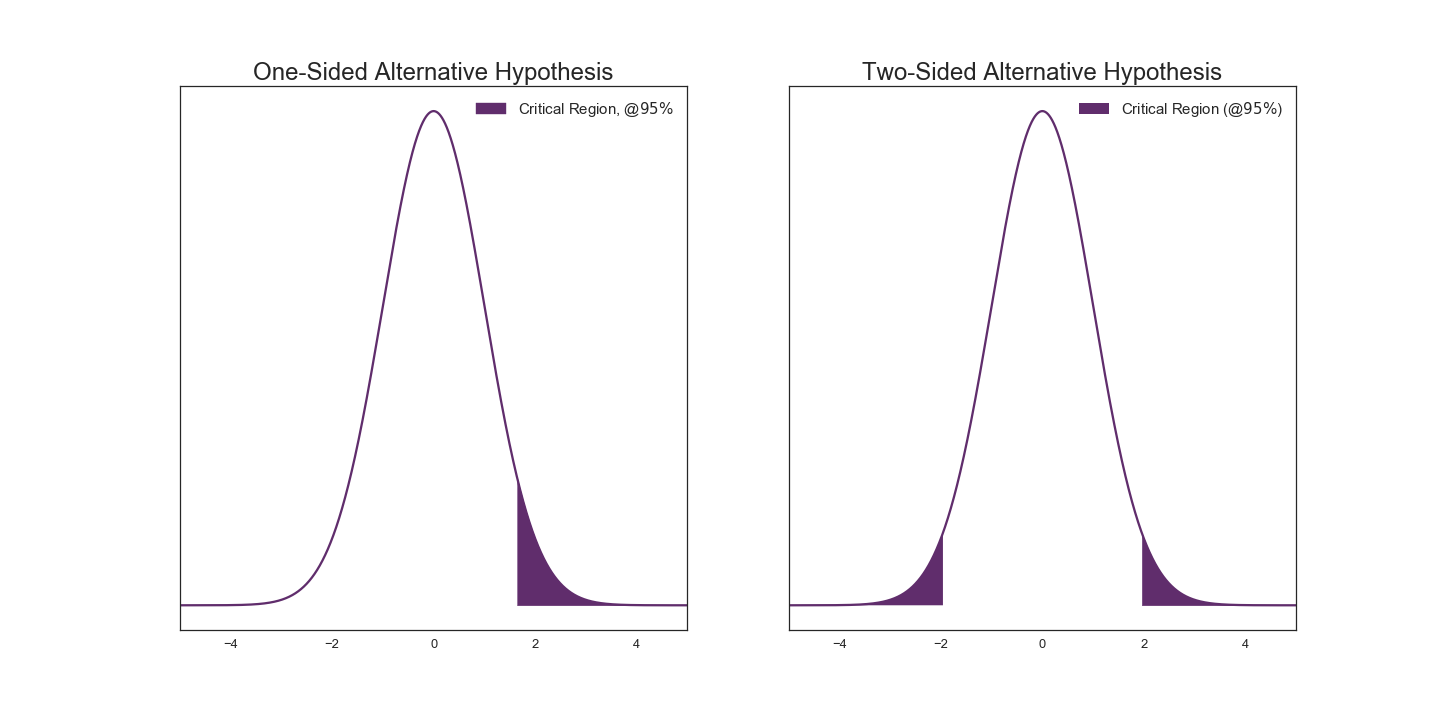
\includegraphics[scale=0.35]{one_two_sided}
	\centering
	\captionsetup{width=0.6\textwidth}
	\caption{\label{fig_one_two_sided} The distribution of $t_Z$, and the critical region for one-sided and two-sided Alternative Hypothesis. The area shaded corresponds to 5\% of the total area under the normal curve. In the left figure (one-sided), the threshold is $t_Z \gtrsim 1.65$, in the right figure, the threshold is $\left|t_Z\right| \gtrsim 1.96$. The distributions here are normal, since we're using $t_Z$. If we had used $t_t$ or $t_W$, the distribution would be Student's $t$ distribution, with the appropriate number of degrees of freedom.}
\end{figure}

The critical region defines a set of values for the test statistic $t$, such that, if the value of $t$ for our test falls inside the critical region, we agree to reject the null hypothesis. Since $t$ is a random number (i.e, it's written in terms of measured quantities, which are inherently uncertain), we expect $t$ to randomly fall in the critical region some of the time. In this case, we commit a Type I error. If we expect a Type I error $a\%$ of the time, then we can have $(1-a)\%$ confidence that we \textit{have not} committed a Type I error.

The confidence level is a quantitative way to communicate how unlikely a measurement is, given the Null Hypothesis. When we quote a result ``at a confidence level of $95\%$'', we're saying ``if there were no effect, we have a one in twenty chance at repeating this result'', or ``if the Null Hypothesis were true, we would measure this result in only one of twenty experiments''. 

Our Alternative Hypothesis generally only specifies a direction, and not a particular value. For example, if we're trying to improve click-through ratio, we may take $\mathcal{H}_1: c_c < c_t$. In this case, you're saying ``The treatment will generally have a better CTR than the control''. You \textit{did not} say anything about the magnitude of the improvement. When you get to the end of the experiment and you find that you can, indeed, reject the Null Hypothesis, you're only saying ``We believe that the treatment drives a higher CTR'', you \textit{are not} saying anything about the size of the effect. Your testing results should be taken as directional.

To find the critical region, we want to know what values of the test statistic occur $a\%$ of the time under the Null Hypothesis. The hypothesis can be one sided or two sided, as in Section \ref{sec_hypothesis}. This will affect how we choose a critical region. 
\begin{itemize}
	\item Suppose that the Alternative Hypothesis is one-sided ($\mathcal{H}_1 : p_c < p_t$), and we want to quote results at $95\%$ confidence using the $Z$ test. Under the Null Hypothesis, we need to find the value of $t_Z$ that we expect to occur $95\%$ if the time. Since we chose $t_Z$ to have mean 0 and unit variance (see Equation (\ref{general_t_stat})), we can use an online calculator\footnote{For example: http://www.wolframalpha.com/widgets/view.jsp?id=540d8e149b5e7de92553fdd7b1093f6d.} or lookup table (see Table \ref{tab_threshold}). For a one-sided Alternative Hypothesis, we need $t_Z \gtrsim 1.65$ to reject the Null Hypothesis at $95\%$ confidence.
	\item If our Alternative Hypothesis were two-sided, the critical region is broken up across the left and right tails of the distribution for $t_Z$ -- the critical region encompasses the largest $2.5\%$ of values for $t_Z$ and the smallest $2.5\%$ of values for $t_Z$. Referring to Table \ref{tab_threshold}, we need $\left| t_Z \right| \gtrsim 1.96$ to reject the Null Hypothesis with $95\%$ confidence.
\end{itemize}
Figure \ref{fig_one_two_sided} demonstrates the critical region in both the one-sided and two-sided case for $t_Z$.

\begin{table}
	\begin{tabular}{c|ccc}
		$a$ & confidence & $\mathcal{H}_1$ & Threshold \\
		\hline
		\hline
		$0.05$ & $95\%$ & $p_c < p_t$ & $t_Z \gtrsim 1.65$ \\
		$0.05$ & $95\%$ & $p_c > p_t$ & $t_Z \lesssim -1.65$ \\
		$0.01$ & $99\%$ & $p_c < p_t$ & $t_Z \gtrsim 2.33$ \\
		$0.01$ & $99\%$ & $p_c > p_t$ & $t_Z \lesssim -2.33$ \\
		\hline
		$0.05$ & $95\%$ & $p_c \neq p_t$ & $\left|t_Z \right| \gtrsim 1.96$ \\\
		$0.01$ & $99\%$ & $p_c \neq p_t$ & $\left|t_Z \right| \gtrsim 2.58$ \\
		\hline	
	\end{tabular}
	\centering
	\captionsetup{width=0.6\textwidth}
	\caption{\label{tab_threshold}  A few critical values of $t_Z$ under one-side/two-sided Alternative Hypotheses.}
\end{table}

\subsection{Statistical Power}

Statistical power is the probability that you've correctly rejected the Null Hypothesis, in the case where the Null Hypothesis is false. Since $b$ is the probability of committing a Type II error, $\mathrm{Power} = 1 - b$. 

It's easiest to demonstrate the concept graphically, see Figure \ref{fig_crit_region}. In this experiment, we are measuring a small effect size on a large amount of traffic (this is the typical case, as in Section \ref{assumptions}), so we've decided to use $t_Z$. We're looking to achieve $95\%$ confidence in our results, and our hypothesis is two-tailed\footnote{Here we're looking at the distribution of the quantity we're measuring, $p_c$ and $p_t$. In Figure \ref{fig_one_two_sided}, we plotted the distribution of the test statistic $t_Z$. Keep in mind that these are two different quantities.}. The control group has $p_c = 61.0\%$. In order to see an effect at $95\%$ confidence, we need $p_t \leq 60.86\%$ or $p_t \geq 61.14\%$. As it turns out, we measure $p_t = 61.15\%$. The critical regions in Figure \ref{fig_crit_region} are the darker purple area in the tails of the distribution for $p_c$, and the statistical power of the test is the lighter blue shaded area. In this experiment, we calculate:
\begin{equation}
	\mathrm{Power} = 59.91\%.
\end{equation}
A few more points about Figure \ref{fig_crit_region}:
\begin{itemize}
	\item Generally, the larger the power, the more confidence we can have that we're not making a Type II error.
	\item $a$ and $b$ cannot be independent. While we can choose $a$ at the onset of the experiment, we cannot calculate $b$ until we've measured $p_c$ and $p_t$.
	\item Power can never be less than $50\%$ if we reject the null hypothesis. It can never be $100\%$ either, just as confidence can never be $100\%$.
\end{itemize}

\begin{figure}[h!]
	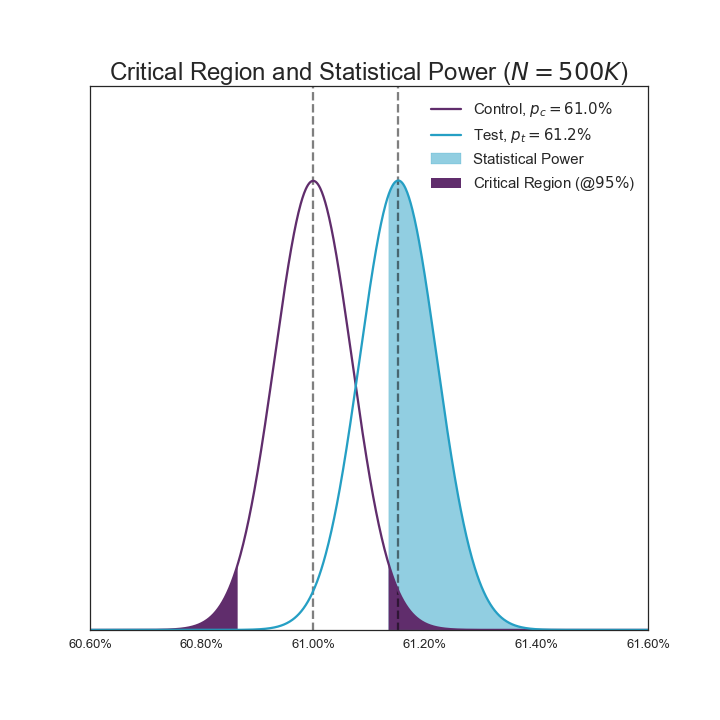
\includegraphics[scale=0.45]{critical_region_and_statistical_power}
	\centering
	\captionsetup{width=0.6\textwidth}
	\caption{\label{fig_crit_region} The ``critical region'' and ``statistical power'' of a simple AB test. Here, the Alternative Hypothesis is two-tailed, $\mathcal{H}_1: p_c \neq p_t$. The critical regions were set such that we can reject the Null Hypothesis with 95\% confidence if $p_t$ falls in one of them. The statistical power corresponds to the ability of the test, given the parameters, to reject the Null Hypothesis. In this experiment, we were able to find a tiny but statistically significant effect ($0.25\%$ relative change) because of the large sample size.}
\end{figure}

\section{Putting it all Together: Experiment Design}

Generally, the test process works as follows:
\begin{itemize}
	\item Product/Engineering build a new experience
	\item Analytics/Product estimate the impact, and Analytics sets the parameters of the experiment.
	\item The experiment runs for a set period of time, with daily check-ins to verify that analytics are firing, and that results are not too bad.
	\item Once results become statistically significant, the test is turned off and the data analyzed. The test may run slightly longer than needed, to ensure that there are no ``close calls''.\footnote{Decisions are hard when $t$ values are right on the line. If you let the test run for a day longer than needed, you'll help to ensure that there will be enough data to suss out a small effect.}
\end{itemize}

\subsection{Calculating Thresholds, Confidence, and Power}

To calculate the threshold:
\begin{enumerate}
	\item Determine if the hypothesis is one-sided or two-sided.
	\item Determine the confidence with which you'd like to quote results.
	\item Determine the statistical test you'd like to run.
	\item Using the appropriate distribution for the test statistic (called $\Phi_{stat}$), determine the threshold that $t$ must satisfy.
\end{enumerate}
For example, suppose we want to use the $Z$ test. The distribution in this case is the standard normal distribution $\Phi_0(x)$ (mean zero, unit variance):
\begin{eqnarray}
	\mathrm{One-tailed:} && \Phi_0(x) = \frac{1}{\sqrt{2\pi}} \int_{-\infty}^x e^{-\frac{t^2}{2}} dt = 1-a\\
	\mathrm{Two-tailed:} && \Phi_0(x) = \frac{1}{\sqrt{2\pi}} \int_{-x}^x e^{-\frac{t^2}{2}} dt = 1-a.
\end{eqnarray}
You don't actually have to calculate these integrals directly, -- Excel, Python (using the scipy package\footnote{For example: https://docs.scipy.org/doc/scipy/reference/generated/scipy.stats.norm.html}), and R all have programmatic ways to calculate these integrals. You can also look them up in books, or find calculators online. For the $Z$ test, a few thresholds are contained in Table \ref{tab_threshold}.

To calculate statistical power:
\begin{enumerate}
	\item Determine the distribution for $p_c$, $\Phi_c(x)$. Determine the cutoffs for the critical region(s).
	\item Determine the distribution for $p_t$, $\Phi_t(x)$.
	\item If the value for $p_t$ falls in the critical region, integrate the distribution for $p_t$ from the relevant critical region to infinity.
\end{enumerate}
In the following, we assume normal distributions for $p_c$ and $p_t$. We also assume that the Alternative Hypothesis is $\mathcal{H}_1 : p_c < p_t$. Then:
\begin{equation}
	\Phi_c(x) = \frac{1}{\sqrt{2\pi}}\int_{-\infty}^x e^{\frac{-(p-p_c)^2}{2\sigma_c^2}} dp.
\end{equation}
The critical value $x_0$ (for $95\%$ confidence) is defined as:
\begin{equation}
	\Phi_c(x_0) = \frac{1}{\sqrt{2\pi}}\int_{-\infty}^{x_0} e^{\frac{-(p-p_c)^2}{2\sigma_c^2}} dp = 0.95.
\end{equation}
Typically, we could look this value up using an inverse normal distribution calculator. Formally, this amounts to evaluating:
\begin{equation}
	x_0 = \Phi_c^{-1}(0.95).
\end{equation}
Now, suppose that we find $p_t > x_0$, as in Figure \ref{fig_crit_region}. Once we determine $p_t$, we can also write down $\Phi_t(x)$. Then we calculate the statistical power as
\begin{equation}
	\Phi_t(x_0) = 1 - \frac{1}{\sqrt{2\pi}} \int_{-\infty}^{x_0} e^{-\frac{(p-p_t)^2}{2\sigma_t^2}} dp.
\end{equation}
As before, there's no need to evaluate these integrals directly. 

\subsection{Traffic Planning}

Generally, tests are not open-ended. The longer a test runs, the more opportunities there are for problems, so we like to have a good sense for when a test \textit{should} end. This is possible because we agree at the onset to a confidence level (say, $95\%$), and an hypothesis.

This is easiest to demonstrate with an example: Suppose we want to run a test to increase click-through ratio $c$. Historically, CTR has hovered around $61\%$, and we estimate that the change we're testing will increase it by $1\%$. We'd like to quote results at $95\%$ confidence, and we're going to use the $Z$ test. 

First, referring to Table \ref{tab_threshold}, we seek $\left| t_Z \right| \gtrsim 1.96$, which we'll round up to 2 for good measure. We use Equation (\ref{alternative_z_stat}) with the following assumptions:
\begin{itemize}
	\item $t_Z = 2$;
	\item $n_c = n_t = n$;
	\item $p_c = 61\%$, $p_t = 61\% \times 1.01 = 61.6\%$.
\end{itemize}
Then:
\begin{eqnarray} \nonumber 
	t_Z = 2 &=& \frac{0.6\%}{\sqrt{\frac{1}{n}\left(0.61 \times 0.39 + 0.616\times 0.384\right)}}  \\ \nonumber
	\sqrt{\frac{1}{n}} &=& \frac{0.006}{1.378} = 4.36 \times 10^{-3} \\
	\Rightarrow n &\approx& 53,000.  
\end{eqnarray}
Thus, we should be able to decipher a relatively small lift in CTR with only 53,000 visits per slice. Keep in mind that this is an estimate -- if the effect size is smaller than anticipated, you'll need more traffic to get more statistical power. The test should run until results become significant and stabilize\footnote{Statistical significance can come and go -- that is, it's entirely possible that results are statistically significant at one moment in time, but that (as more data comes in), the results are no longer statistically significant. Generally this isn't too much of an issue, and if you notice this happening, you'll want to let the test run a bit longer.}.

\end{document}